\documentclass{scrartcl}

\usepackage[english]{babel}
\usepackage[utf8]{inputenc}
\usepackage{mathtools}
\usepackage{fancyvrb}
\usepackage{graphicx}
\usepackage{caption}
\usepackage{subcaption}

%\usepackage{minted}

\fvset{xleftmargin=2em} % Indryk all fancyvrb kode lister

\newcommand\code[1]{\texttt{#1}}

\begin{document}

%\newminted{java}{linenos, obeytabs, tabsize=2}

\title{Assignment 4}
\subtitle{02102 Introductory Programming}
\author{
  Daniel Safari\\
  \texttt{s134110}
  \and
  Troels Mæhl Folke\\
  \texttt{s134061}
   \and
  Henrik Enggaard Hansen\\
  \texttt{s134099}
}
\date{6/4/2014}
\maketitle
\thispagestyle{empty}
\setcounter{page}{0}
\null
\vfill
\section*{Work distribution}

Each member had the main responsibility for one problem, but all members
actively contributed with comments and suggestions for all problems. 
The exact distribution was as following:
\begin{itemize}
\setlength{\itemindent}{3em}
\item[Problem 1:] xxx
\item[Problem 2:] Daniel Safari
\item[Problem 3:] xxx
\item[Paper:]  All
\end{itemize}
\newpage

\section*{Problem 1}

The task was to implement classes for representing literary references. Using
classes as abstractions it should be possible for the \code{Artikel}-class to
have instances of other \code{Artikel}s which in turn have instances of
\code{Tidsskrift} and in turn of \code{Forlag}.

When an \code{Artikel}-class is correctly instantiated and set up, passing it
to \code{print} (or calling \code{.toString}) yields the following output:
\begin{Verbatim}
"A" by A. Abe & A. Turing

References:
B. Bim: B, Brain, University Press, Denmark
\end{Verbatim}

\section*{Problem 2}
The Mandelbrot set consists of the complex numbers whose sizes do not increase beyond two despite the amount of iterations of the following algorithm they undergo:

\[ z_{1} = (z_{0})^2 + z_{0}  \]
\[ z_{2} = (z_{1})^2 + z_{0}  \]
\[ z_{3} = (z_{2})^2 + z_{0}  \]
\[ z_{4} = (z_{3})^2 + z_{0}  \]
\[ \vdots \]

The accuracy of this algorithm naturally depends on the maximum amount of iterations we're willing do.
Plotting complex number that belong to the Mandelbrot set in the complex plane and zooming in on the edges leads to repeating patterns, fractals.
Coloring each point in the complex plane according to amount of iterations undergone leads to interesting visuals, compared to merely coloring a point if it is determined to belong to the Mandelbrot set.

In order to plot the Mandelbrot set, the following steps must be carried out:
\begin{enumerate}
\item Define a grid of points on the screen
\item Iterate each point until we reach the \code{MAX} number of iterations or the length of $z_{i}$ exceeds two
\item Color each point the color corresponding to the number of iterations undergone
\end{enumerate}

In the case of our program, the \code{gridSize} is set by the user upon \code{initialization}.
The desired \code{palette}, \code{width} and \code{centerDot} is also set upon \code{initialization}.
Once our program has been initialized, the function \code{drawFractals} is called.
\code{drawFractals} draws each point in the grid in the color which \code{palette} specifies for the number of iterations the relevant point undergoes. 

Once the initial drawing has been completed, the function \code{navigation}, which alters the current viewport, runs for the remainder of the program's runtime; continuously pooling keypresses. The amount of zoom and movement \code{navigation} applies for each keypress is determined by the constants \code{MOVEFACTOR} and \code{ZOOMFACTOR}.

\newpage
Test run 1:
\begin{Verbatim}
Welcome to Mandelbrot navigator, use WASD for navigation and Q/E for zoom.
Multicolor? (y/n): yes
Color from file? (y/n): yes
Please enter file path of color file: blues.mnd
Input the real part of the center coordinate (if unsure, use 0): 0,10684
Input the imaginary part of the center coordinate (if unsure, use 0): -0,63675
Input the width of the coordinate system (if unsure, use 2): 0,0085
Input desired grid size (use low grid size for smooth navigation): 1000
\end{Verbatim}

Test run 2:
\begin{Verbatim}
Welcome to Mandelbrot navigator, use WASD for navigation and Q/E for zoom.
Multicolor? (y/n): no
Input the real part of the center coordinate (if unsure, use 0): -0,5
Input the imaginary part of the center coordinate (if unsure, use 0): 0
Input the width of the coordinate system (if unsure, use 2): 2
Input desired grid size (use low grid size for smooth navigation): 1024
\end{Verbatim}

Test run 3:
\begin{Verbatim}
Welcome to Mandelbrot navigator, use WASD for navigation and Q/E for zoom.
Multicolor? (y/n): yes
Color from file? (y/n): no
Input the real part of the center coordinate (if unsure, use 0): 0,10087
Input the imaginary part of the center coordinate (if unsure, use 0): -0,63198
Input the width of the coordinate system (if unsure, use 2): 0,0003
Input desired grid size (use low grid size for smooth navigation): 1024
\end{Verbatim}



\begin{figure}
        \centering
        \begin{subfigure}[b]{0.3\textwidth}
                
\includegraphics[width=\textwidth]{filecolor}
                \caption*{First rest run}
        \end{subfigure}%
        ~
        \begin{subfigure}[b]{0.3\textwidth}
                
\includegraphics[width=\textwidth]{nocolor}
                \caption*{Second test run}
        \end{subfigure}
         ~
        \begin{subfigure}[b]{0.3\textwidth}
                
\includegraphics[width=\textwidth]{randomcolor}
                \caption*{Third test run}
        \end{subfigure}
\end{figure}


\section*{Problem 3}

The task is to implement John Horton Conway's Game of Life.

The solution is structured as a front-end class \code{GameOfLifeMain} which
handles input and output and a backend class \code{GameOfLife} which handles
the game logic.

When \code{GameOfLife} is instantiated, the \emph{world} is setup. The world
is represented as a two dimensional array of integers. This two dimesional
array can also be provided, in such a case all rows must be the same length as
the number of columns -- it must be a square.

On this instance of the class (the Game of Life World) the method
\code{nextState} calculates the next state of all cells in the world. To do
this the method \code{liveNeighbours} is used. \code{LiveNeighbours}
calculates the number of live neighbouring cells to a point in the world. The
method accounts for over- and underflowing the coordinate system. If a
neighbour is past the right edge of the world, the coordinate is instead set
the neighbour on the left edge. This gives the world the topology of a torus.

Random noise can be introduced to world using the method \code{cosmicNoise}.
The method takes an argument $p$ which is the probability a cell has toggling
state. 
\begin{figure}
        \centering
        \begin{subfigure}[b]{0.3\textwidth}
				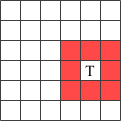
\includegraphics{Normal-target}
                \caption*{A normal target}
        \end{subfigure}%
        ~
        \begin{subfigure}[b]{0.3\textwidth}
				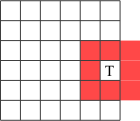
\includegraphics{Off-target}
                \caption*{A targer with overlapping}
        \end{subfigure}
         ~
        \begin{subfigure}[b]{0.3\textwidth}
				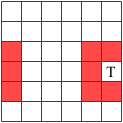
\includegraphics{Off-target-adjusted}
                \caption*{Adjusted neighbour cells}
        \end{subfigure}
\end{figure}

Running the program

\begin{Verbatim}
java GameOfLife
\end{Verbatim}

With file input

\begin{Verbatim}
java GameOfLife glider_gun.gol
\end{Verbatim}


\includegraphics[width=0.5\textwidth]{gol-example}

\end{document}
